\documentclass{beamer}
%\usetheme{}%\usecolortheme{}
\setbeamertemplate{navigation symbols}{}
\setbeamertemplate{section in toc}[sections numbered]
\setbeamertemplate{footline}[frame number]

\usepackage[utf8]{inputenc}
\usepackage[T1]{fontenc}
\usepackage{lmodern}
\usepackage{appendixnumberbeamer}
\usepackage{multirow}

\title{%
  \textbf{BEST: a Binary Executable Slicing Tool}
  \\ and its use to improve
  \\ Model Checking-based WCET Analysis}
\author{%
  \textbf{Armel Mangean}$^1$
  \and Jean-Luc Béchennec$^2$
  \and Mikaël Briday$^3$
  \and Sébastien Faucou$^3$}
\institute{%
  IRCCyN, UMR CNRS 6597
  \\ $^1$École Centrale de Nantes, $^2$CNRS , $^3$Université de Nantes}
\date{July 5, 2016}

% 20 min -> ~15 slides

\begin{document}

  \begin{frame}
    \titlepage

    \begin{center}
      \includegraphics[height=0.8cm]{fig/irccyn.png}
    \end{center}

    \emph{\small 16th International Workshop on Worst-Case Execution Time Analysis}
  \end{frame}

  \begin{frame}
    \frametitle{~}
    \tableofcontents
  \end{frame}

  %%%
  
  \section{Introduction}
  \begin{frame}
    \frametitle{\secname}
    \tableofcontents[currentsection]
  \end{frame}
  
  \subsection{Motivation}
  \begin{frame}
    \frametitle{\secname}
    \framesubtitle{\subsecname}
    
    \begin{figure}
      \centering
      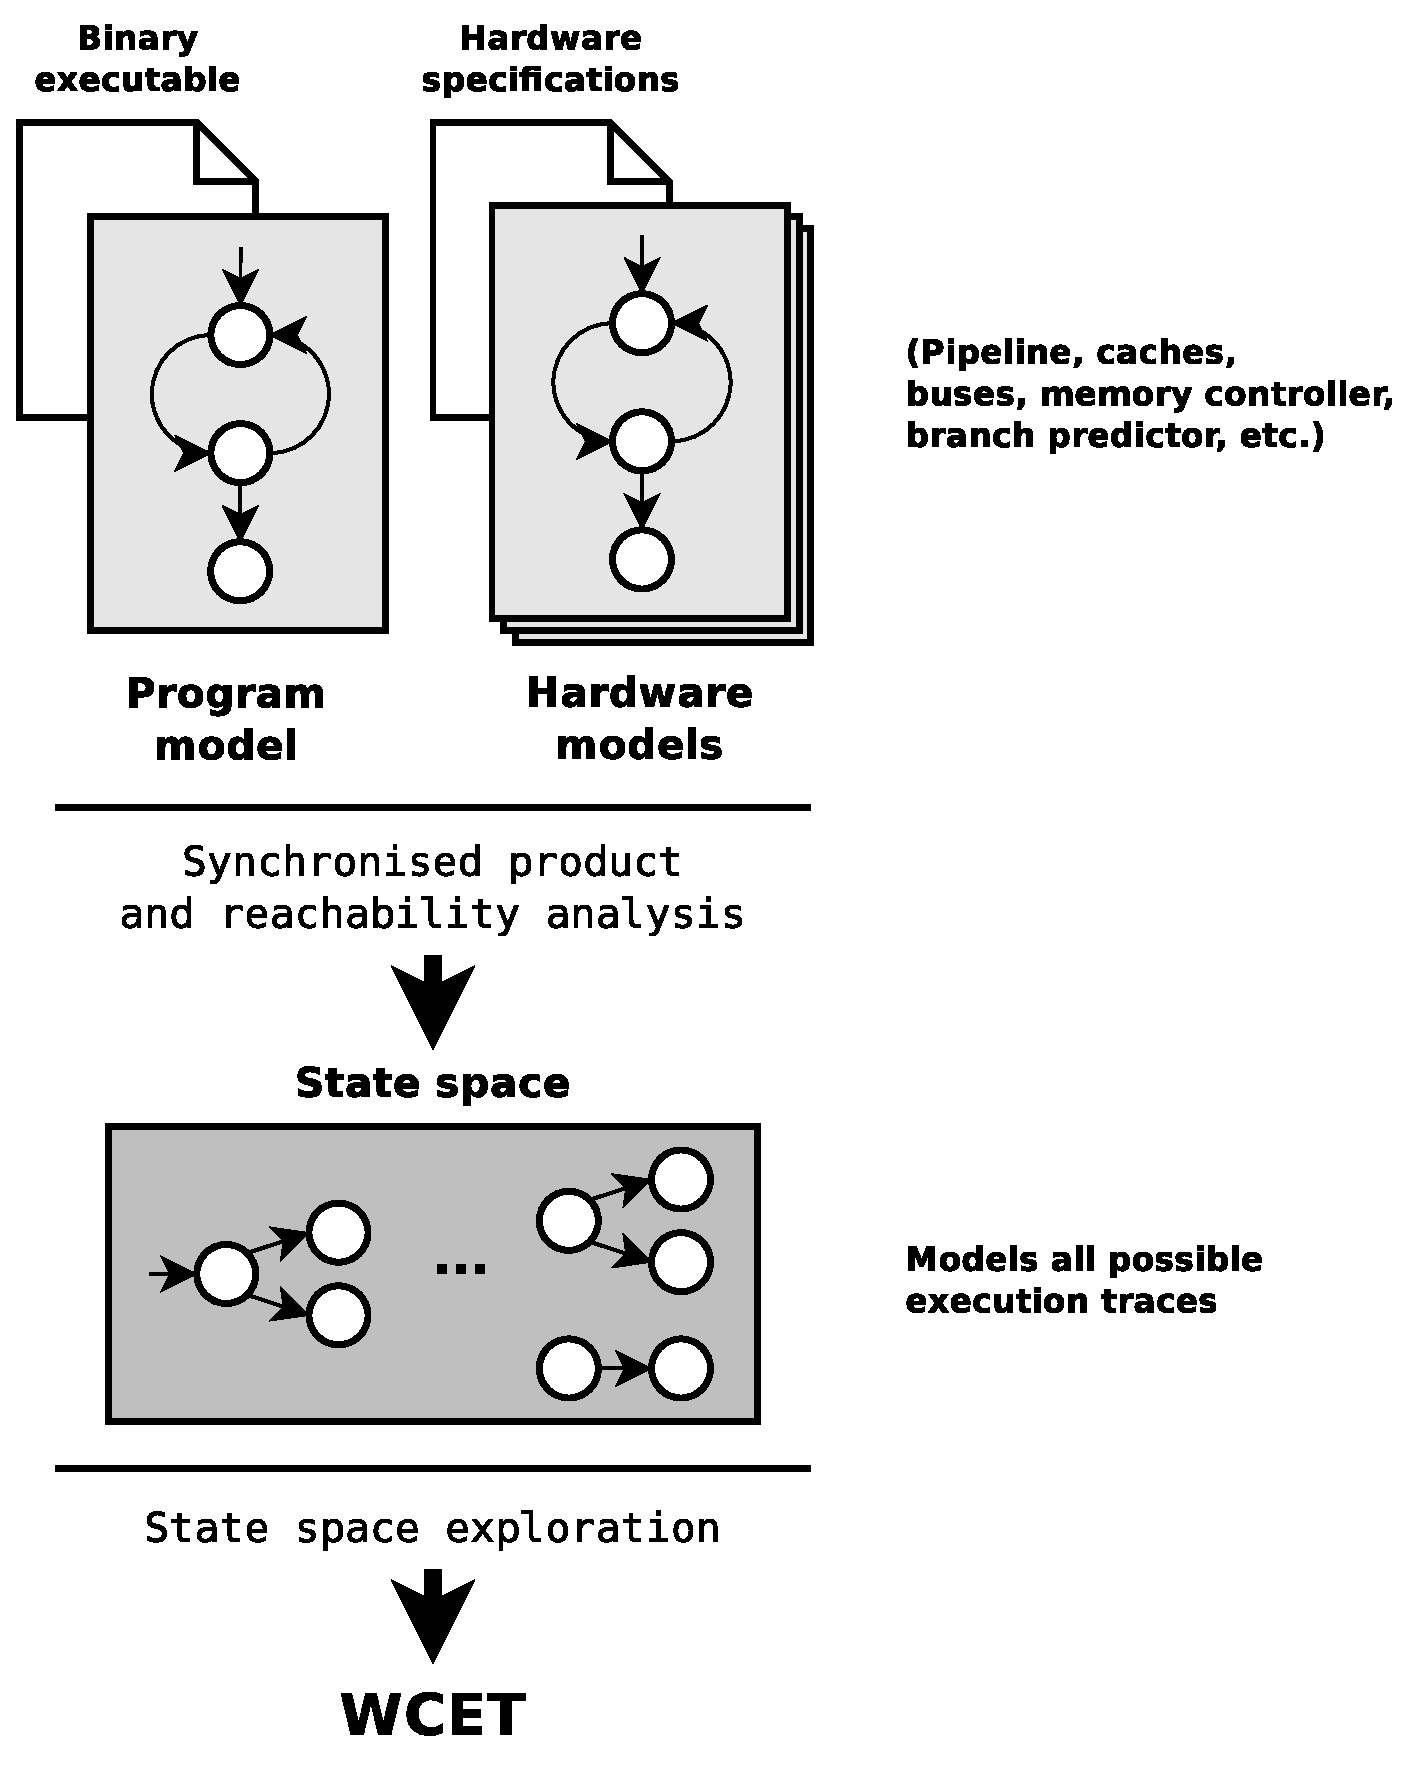
\includegraphics[height=.85\textheight]{fig/model-checking.eps}
    \end{figure}
  \end{frame}

  \begin{frame}
    \frametitle{\secname}
    \framesubtitle{\subsecname}
    
    \begin{block}{Motivation:}
        \begin{description}
          \item[modularity] network of timed automata
          \item[tightness] exact cache analysis
            \begin{itemize} % infeasible with AI
            \item arbitrary cache policy (not only LRU nor PLRU)
            \end{itemize}

          \vspace{1em}
          \item[witnesses] initial hardware and software states
          \item[binary level] no high level source code analysis
        \end{description}
    \end{block}
  \end{frame}
  
  \subsection{Challenge}
  \begin{frame}
    \frametitle{\secname}
    \framesubtitle{\subsecname}
      
    \begin{block}{Limitations:}
      \begin{itemize}
        \item suffer of the state space explosion
        \item tailored for embedded microcontrollers % but thus precise
      \end{itemize}
    \end{block}
    
    \vspace{1em}
    \begin{block}{Challenges:}
      \begin{itemize}
        \item abstracting models of hardware components~\cite{CGM15}
        \item \textbf{abstracting models of programs}~\cite{BJ14,CB13,MBB16}
      \end{itemize}
    \end{block}
  \end{frame}

  %%%

  \section{Program Abstraction using Program Slicing}
  \begin{frame}
    \frametitle{\secname}
    \tableofcontents[currentsection]
  \end{frame}

  \subsection{Overview of Program Slicing}
  \begin{frame}
    \frametitle{\secname}
    \framesubtitle{\subsecname}

    \begin{itemize}
      \item a program $P \subseteq L \times I$ with
        \begin{itemize}
          \item $L$ a finite set of labels
          \item $I$ a finite set of instructions
          \item $\forall (l,i), (l,i') \in P, i = i'$
        \end{itemize}
      \item $V_P$ the finite set of variables of $P$

      \vspace{1em}
      \item introduced by Weiser in 1981~\cite{Wei81}
      \item a criterion $C = (l,v)$ with
        \begin{itemize}
          \item $l \in L$ a label and
          \item $v \in V_P$ a subset of variables
        \end{itemize}
      \item a slice $S_C \subseteq P$
        \begin{itemize}
          \item same behavior as $P$ wrt. criterion $C$
        \end{itemize}
    \end{itemize}
  \end{frame}
  
  \begin{frame}
    \frametitle{\secname}
    \framesubtitle{\subsecname}

    \vspace{1em}
    \begin{figure}
      \centering
      \begin{overlayarea}{\textwidth}{\textheight}
        \only<1>{\includegraphics[scale=1.4]{fig/fibcallO2-01.pdf}}
        \only<2>{\includegraphics[scale=1.4]{fig/fibcallO2-02.pdf}}
        \begin{center}
          Slicing criterion: $C = ( 3030, \{ctr\} )$
        \end{center}
      \end{overlayarea}
    \end{figure}
  \end{frame}
  
  \begin{frame}
    \frametitle{\secname}
    \framesubtitle{\subsecname}
    
    \begin{itemize}
      \item dataflow equation-based or graph-based
        \begin{itemize}
          \item fixpoint computation or
          \item reachability analysis
        \end{itemize}
        
      \vspace{1em}
      \item slicing binary executables
      \begin{itemize}
        \item a closed issue~\cite{KJL03} (although not trivial)
        \item multiple graph computation from a CFG
        \item reachability analysis on the final graph
      \end{itemize}
      
      %% \vspace{1em}
      %% \item intuition
      %% \begin{itemize}
      %%   \item the Control Flow Graph
      %%   \item a Control Dependence Graph (of basic blocks)
      %%   \item a Data Dependence Graph (of instructions)
      %%   \item a summary Program Dependence Graph
      %% \end{itemize}
    \end{itemize}
  \end{frame}
  

  \subsection{Abstracting models of programs}
  \begin{frame}
    \frametitle{\secname}
    \framesubtitle{\subsecname}

    \begin{figure}
      \centering
      \includegraphics[height=.85\textheight]{fig/example.png}
    \end{figure}

    %% \begin{itemize}
    %%   \item how to abstract models of program using program slicing?
    %%   \item removing instructions would results in losing essential information
    %%     regarding registers use and thus pipeline timing behavior.
    %%   \item so we can't remove instructions

    %%   \item what can we remove?
        
    %%   \item How do we use Program Slicing to abstract models of programs?
      
    %%   \vspace{1em}
    %%   \item Abstracted models of programs keep the same time behaviour as
    %%     unabstracted models.
    %%   \item We do not intend to perform WCET analysis on slices but on abstracts
    %%     models of programs built using information gathered through program
    %%     slicing.
    %%   \item Instructions not in the slice are abstracted (not removed, they keep
    %%     their time behaviour) others are not.
    %% \end{itemize}
  \end{frame}

  \subsection{Tool implementation}
  \begin{frame}
    \frametitle{\secname}
    \framesubtitle{\subsecname}

    \begin{figure}
      \centering
      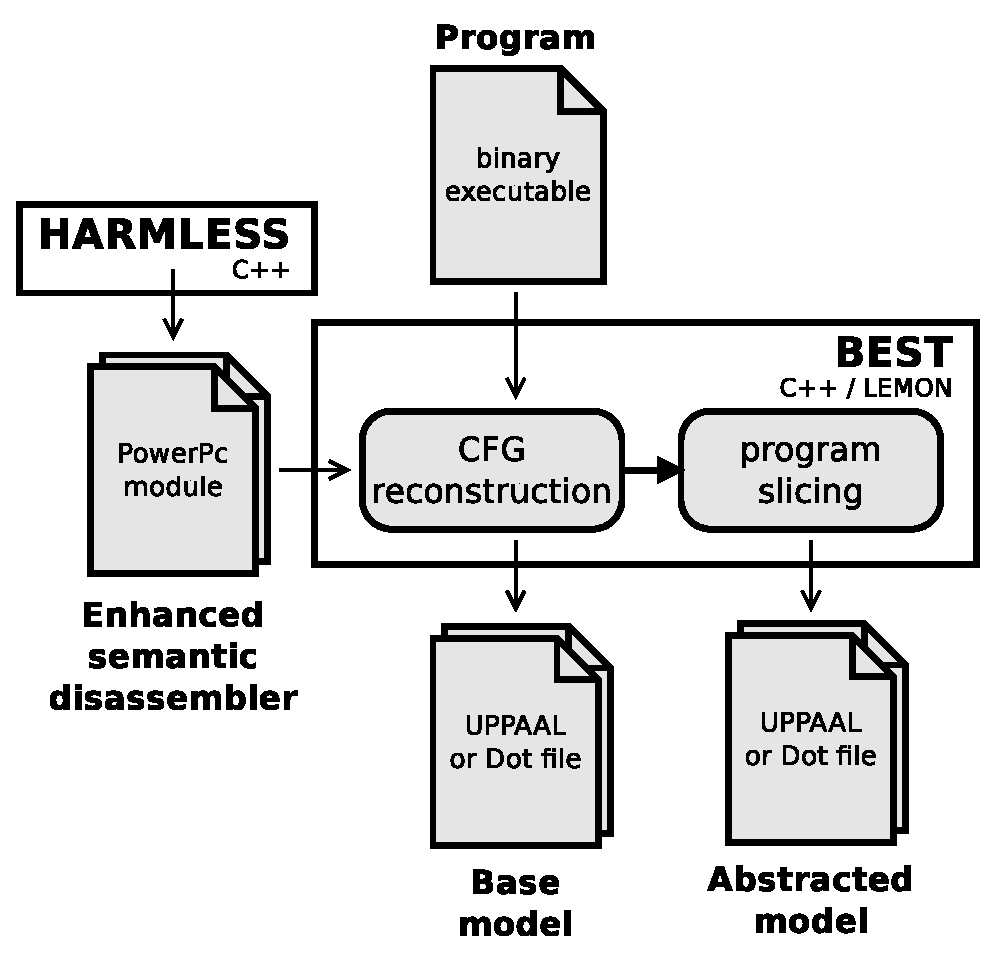
\includegraphics[height=.85\textheight]{fig/archi.eps}
    \end{figure}
  \end{frame}

  %%%
  
  \section{Experimental results}
  \begin{frame}
    \frametitle{\secname}
    \tableofcontents[currentsection]
  \end{frame}
  
  \subsection{Methodology}
  \begin{frame}
    \frametitle{\secname}
    \framesubtitle{\subsecname}

    \begin{itemize}
      \item use of Mälardalen WCET benchmarks
      \item excluding programs containing % 16 out of the 35
        \begin{itemize}
          \item switch-case statements % whereas it's a closed issue
          \item floating-point arithmetic % missing in the PowerPC HADL file 
          \item recursive programs
        \end{itemize}
      \item multiple compilers and optimisation options
        \begin{itemize}
          \item \textsc{Gcc} 5.3.1 (\texttt{-O0}, \texttt{-O1}, \texttt{-O2}, \texttt{-O3})
          \item \textsc{Cosmic C} 4.3.7 (\texttt{-no}, \emph{default})
          \item targeting the PowerPC 32 bits instruction set
        \end{itemize}
      \item sums up to 96 binaries

      \vspace{1em}
      \item use of Trampoline RTOS~\cite{BBF06} services
        \begin{itemize}
          \item not documented on our paper
        \end{itemize}
    \end{itemize}
  \end{frame}
  
  \subsection{Results}
  \begin{frame}
    \frametitle{\secname}
    \framesubtitle{\subsecname}

    \begin{table}
      \centering
      \tiny
      \begin{tabular}{ |l| |c|c|c|c| |c|c| }
    \hline
      \multirow{2}{*}{Source file}
    & \multicolumn{4}{c||}{\textsc{Gcc}}
    & \multicolumn{2}{c|}{\textsc{Cosmic}}
      
  \\\cline{2-7}
    & \emph{default} & \verb|-O1|     & \verb|-O2| & \verb|-O3|
    & \verb|-no|     & \emph{default}

  \\\hline
      \verb|adpcm.c|
    & -32\% (19) & -12\% (34) & -7\% (30) & -8\% (38)
    & -38\% (39) & -38\% (39)

  \\\hline
      \verb|bs.c|
    & -31\% (13) & -23\% (13) & -10\% (10) & -10\% (10)  
    & -29\% (14) & -15\% (13)

  \\\hline
      \verb|bsort100.c|
    & -21\% (14) & -25\% (20) & -31\% (16) & -31\% (16)
    & -13\% (15) & -13\% (15)
      
  \\\hline
      \verb|cnt.c|
    & -29\% (17) & -25\% (20) & -38\% (16) & -40\% (20)  
    & -69\% (39) & -69\% (39) 

  \\\hline
      \verb|compress.c|
    & -19\% (21) & -15\% (33) & -9\% (35) & -8\% (37)  
    & -41\% (39) & -41\% (39) 

  \\\hline
      \verb|crc.c|
    & -47\% (19) & -36\% (25) & -52\% (21) & -57\% (21)
    & -49\% (39) & -49\% (39) 

  \\\hline
      \verb|expint.c|
    & -33\% (15) & -36\% (28) & -64\% (11) & -64\% (11)  
    & -59\% (39) & -59\% (39) 

  \\\hline
      \verb|fdct.c|
    & -47\% (15) & -83\% (23) & -88\% (32) & -91\% (35)
    & -92\% (37) & -92\% (37)

  \\\hline
      \verb|fibcall.c|
    & -31\% (13) & -42\% (12) & -57\% (7) & -57\% (7) 
    & -50\% (12) & -40\% (10) 

  \\\hline
      \verb|fir.c|
    & -50\% (18) & -38\% (24) & -30\% (23) & -30\% (23)
    & -56\% (39) & -56\% (39) 

  \\\hline
      \verb|janne_complex.c|
    & -36\% (14) & -33\% (9) & -25\% (8) & -22\% (9) 
    & -82\% (38) & -13\% (8) 

  \\\hline
      \verb|jfdctint.c|
    & -23\% (13) & -80\% (15) & -85\% (27) & -89\% (35)
    & -92\% (37) & -92\% (37) 
      
  \\\hline
      \verb|matmult.c|
    & -43\% (21) & -23\% (22) & -19\% (21) & -29\% (21)
    & -74\% (39) & -74\% (39) 
      
  \\\hline
      \verb|ndes.c|
    & -42\% (19) & -21\% (29) & -11\% (28) & -3\% (30)  
    & -54\% (39) & -56\% (39) 
      
  \\\hline
      \verb|ns.c|
    & -31\% (16) & -24\% (17) & -13\% (15) & -25\% (12)  
    & -59\% (39) & -58\% (38) 
      
  \\\hline
      \verb|prime.c|
    & -20\% (15) & -33\% (9) & -33\% (9) & -25\% (8)   
    & -66\% (38) & -63\% (38) 
      
  \\\hline
\end{tabular}

    \end{table}
    
    \begin{itemize}
      \item execution time negligible (always < 1 sec.)
    \end{itemize}
  \end{frame}

  %%%
  
  \section{Future work}
  \begin{frame}
    \frametitle{\secname}
    \tableofcontents[currentsection]
  \end{frame}
  
  \begin{frame}
    \frametitle{\secname}

    \begin{itemize}
      %\item can not account for indirect branch
      \item adapt to interprocedurality (straightforward)
      \item extending to stack frames and initialized data
      \begin{itemize}
        \item bigger slices but not necessarily bigger state space
      \end{itemize}

      \vspace{1em}
      \item modeling the PowerPC e200z4 core
        \begin{itemize}
          \item no data cache
          \item instruction cache
            \begin{itemize}
              \item 2 or 4-ways associative
              \item pseudorandom (global FIFO)
            \end{itemize}
          \item branch prediction, \dots
        \end{itemize}
      \item modeling the MPC5643L microcontroller
        \begin{itemize}
          \item two PowerPC e200z4 cores
          \item XBAR crossbar switch
            \begin{itemize}
              \item multiple masters / multiple slaves
              \item possible fixed priority policy % between masters
            \end{itemize}
        \end{itemize}

      \vspace{1em}
      \item (parallel) WCET analysis
    \end{itemize}
  \end{frame}

  %%%

  \section*{Conclusion}
  \begin{frame}
    \frametitle{\secname}
    \framesubtitle{\subsecname}

    \begin{itemize}
    \item abstract models of program
      \begin{itemize}
        \item for Model Checking-based WCET analysis
        \item based on program slicing
      \end{itemize}
      
    \vspace{1em}
    \item a binary executable slicing tool
      \begin{itemize}
        \item instruction set independant
        \item free sofware
        \item promising experimental results
      \end{itemize}

    \vspace{1em}
    \item further work
        
      %  \begin{itemize}
      %    \item compiler knowledge independent
      %    \item instruction set independent
      %  \end{itemize}
      %\item thanks to (a re-targeting of) HARMLESS
      %  \begin{itemize}
      %    \item primarly a generator of cycle accurate simulators
      %    \item based on a hardware architecture description language (HADL)
      %  \end{itemize}

      %\vspace{1em}
      %\item free software under General Public License % free as in freedom
      %\item written in C++ and using LEMON~\cite{DJK11}
      %\item outputs textual, Graphviz and UPPAAL files
    \end{itemize}
  \end{frame}
  
  %%%
  
  \appendix
  \section{References}
  \begin{frame}[allowframebreaks]
    \frametitle{\secname}
    \tiny
    
    \bibliographystyle{plain}
    \bibliography{src/refs.bib}
  \end{frame}
  
\end{document}
